\scanpage{16}
\figure{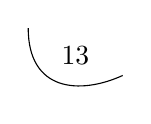
\begin{tikzpicture}[x=1cm,y=1cm]
\node at (0,0) {\mspage{13}};
\draw (-.6,.35) .. controls (-.6,-.45) and (.05,-.5) .. (.6,-.25);
\end{tikzpicture}}
appliquant $\mathbf L_0$ sur $L$, \inserted{et les $\boldsymbol\pi_i$ en les $\pi_i$ \deleted{$\unsure{\pi_i}$} (donc $\pi_i\in\mathcal E$)}.
\deleted{\unsure{respectant la graduation de} $\mathcal E$ \unsure{par les} $\pi_i$}.
\margin{\figure{
\begin{tikzpicture}
\node[align=center] at (0,0) {condition\\essentielle !};
\draw (0,0) ellipse (1.65cm and .9cm);
\draw (-1,.6)--(.1,.7);
\end{tikzpicture}}}

De plus, sous ces conditions, l'hom. annoncé \deleted{\unsure{quelque}} dans (ii) est unique, et avec les notations du n\textsuperscript{o} 6, il transforme $\boldsymbol\Lambda_0$ en $\Lambda$, les \deleted{$\unsure{\pi_{i\alpha}}$} $\boldsymbol\pi_{i\alpha}$ en $\pi_{i\alpha}$, $\boldsymbol\pi_i$ en $\pi_i$, $\boldsymbol\varphi_i^{\beta,\alpha}$ en $\varphi_i^{\beta,\alpha}$ \deleted{$\unsure{\varphi_{i,\alpha}^{j,\beta}}$}.
\margin{\figure{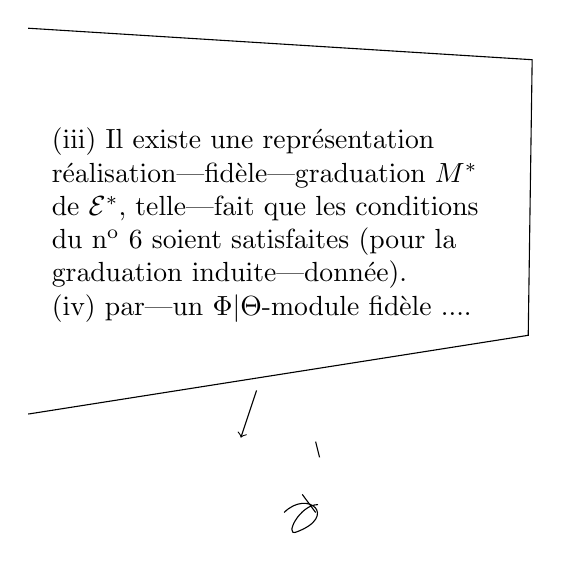
\begin{tikzpicture}
\node[align=left,text width=5.8cm] at (0,0) {(iii) Il existe une \deleted{\unsure{représentation}} \uline{\unsure{réalisation|fidèle|graduation}} $M^*$ de $\mathcal E^*$, \unsure{telle|fait} que les conditions du n\textsuperscript{o} 6 soient satisfaites (pour la graduation \unsure{induite|donnée}).\\(iv) \unsure{par|un} $\uline{\unsure{\Phi|\Theta}}$-module fidèle ....};
\draw (-3.2,2.5)--(3.2,2.1)--(3.15,-1.4)--(-3.2,-2.4);
\draw[->] (-.3,-2.1)--(-.5,-2.7);
\draw (.45,-2.75)--(.5,-2.95);
\draw (.05,-3.65) .. controls (.35,-3.35) and (.75,-3.7) .. (.2,-3.9) .. controls (.05,-3.95) and (.25,-3.55) .. (.48,-3.55);
\draw (.28,-3.42)--(.45,-3.65);
\end{tikzpicture}}}

\uline{Dém} $(i)\Rightarrow(ii)$ Résulte de la table de multiplication des $\varphi_i^{\beta,\alpha}$ donnée au n\textsuperscript{o} 6, et du th. donné au n\textsuperscript{o} 6.

$(ii)\Rightarrow(i)$ \deleted{Soient $\pi'_i$ les images des $\boldsymbol\pi_i$. On a
\[
\text{\unsure{avec}}\qquad L^\alpha\pi'_i=\pi'_{i+\alpha}L^\alpha
\]
\unsure{voit donc} que les $\pi'_i$ définissent la graduation de $\mathcal E$, parce que ils sont de degré $\unsure{0}$.
Je dis que $\pi'_i=\pi_i$ pour tt $i$. Cf Proposition ci-dessous pour ce point, appliquée à $\Phi\longrightarrow\operatorname{End}(M^*)$.}

Comme on a, pour tt $i\leq n$
\[
(\boldsymbol\Lambda_0^{n-i}\mathbf L_0^{n-i}-1)\boldsymbol\pi_i=0,\qquad
(\mathbf L_0^{n-i}\boldsymbol\Lambda_0^{n-i}-1)\boldsymbol\pi_{2n-i}=0
\]
on en conclut, appliquant $\varphi$ (et posant $\Lambda'=\varphi(\unsure{\boldsymbol\Lambda|\boldsymbol\Lambda_0})$)
\[
(\Lambda'^{n-i}L^{n-i}-1)\pi_i=0,\qquad(L^{n-i}\Lambda'^{n-i}-1)\pi_{2n-i}=0.
\]
Donc la condition (ii) du th. du n\textsuperscript{o} 6 est vérifiée, donc aussi la condition (i).

Pour l'unicité de $\varphi$, \deleted{\unsure{et les propriétés}}\inserted{il suffit} \deleted{\unsure{et les relations}} de voir que $\varphi(\unsure{\boldsymbol\Lambda|\boldsymbol\Lambda_0})=\Lambda$, et \inserted{\unsure{pour} $\varphi(\boldsymbol\pi_{i,\alpha})=\pi_{i,\alpha}$,} \deleted{\unsure{pour ceci}} \deleted{\unsure{Pour} $\varphi(\unsure{\boldsymbol\Lambda})$} compte tenu de $\varphi(\boldsymbol\pi_i)=\pi_i$, \deleted{\unsure{donc on a}} la caractérisation \inserted{\figure{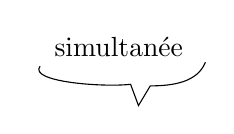
\begin{tikzpicture}[x=1cm,y=1cm]
\node at (0,.4) {simultanée};
\draw (-1,.15) .. controls (-1.15,-.05) and (-.2,-.12) .. (.15,-.08) --(.25,-.35)--(.4,-.1) .. controls (.7,-.1) and (1.0,-.05) .. (1.1,.2);
\end{tikzpicture}}} de $\Lambda$ \inserted{\figure{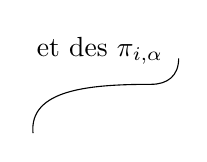
\begin{tikzpicture}[x=1cm,y=1cm]
\node at (.05,.45) {et des $\pi_{i,\alpha}$};
\draw (-.8,-.6) .. controls (-.85,-.05) and (-.1,.02) .. (.7,.02) .. controls (.9,.02) and (1.05,.12) .. (1.05,.35);
\end{tikzpicture}}} par les formules $(\unsure{6.14})$.
\mspage{15}
